\documentclass{article}
\usepackage{amssymb}
\usepackage{pgfplots}
\usepackage{tikz}
\usetikzlibrary{shapes.geometric}
\tikzset{every node/.style={shape=rectangle}}
\begin{document}

\begin{figure}[htbp]
    \centering
    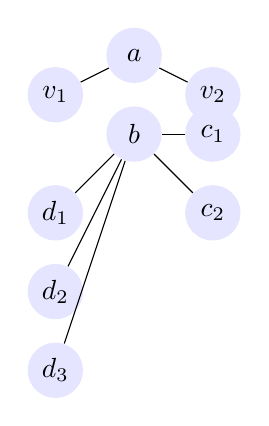
\begin{tikzpicture}
        \tikzstyle{vertex}=[circle,fill=blue!10,minimum size=20pt,inner sep=0pt]
        \node[vertex] (a) at (-1,-0.5) {$v_{1}$};
        \node[vertex] (b) at (0,0) {$a$};
        \node[vertex] (c) at (1,-0.5) {$v_{2}$};

        \node[vertex] (d) at (-1,-2) {$d_{1}$};
        \node[vertex] (e) at (-1,-3) {$d_{2}$};
        \node[vertex] (f) at (-1,-4) {$d_{3}$};

        \node[vertex] (g) at (0,-1) {$b$};
        \node[vertex] (h) at (1,-1) {$c_{1}$};
        \node[vertex] (i) at (1,-2) {$c_{2}$};

        \draw[-] (a) -- (b);
        \draw[-] (b) -- (c);

        \draw[-] (d) -- (g);
        \draw[-] (e) -- (g);
        \draw[-] (f) -- (g);

        \draw[-] (g) -- (h);
        \draw[-] (g) -- (i);

        \end{tikzpicture}
    \caption{}
    \label{}
\end{figure}

\end{document}